\documentclass[letterpaper, 12pt]{article}
\usepackage[francais]{babel}

\usepackage{amsmath,amsfonts,amsthm,amssymb, graphicx,wasysym,multirow}
\usepackage[latin1]{inputenc}

\pagestyle{plain}

\setlength{\topmargin}{-2cm}
\setlength{\textheight}{23.5cm}
\setlength{\textwidth}{18cm}
\setlength{\oddsidemargin}{-1cm}
\setlength{\parindent}{0pt}

%\pdfoutput=1

\begin{document}

2000-- What is the name of a set of people, objects or events on which a statistical study is based? \\

a$)$ A sample \\
b$)$ A population \\
c$)$ A city \\
d$)$ A group \\

Answer: b$)$ \\

Explanation:\\
We are looking for the name of a set of people, objects or events on which a statistical study is based. \\

\begin{itemize}
 \item A sample is a subset of a set of people, objects or events on which a statistical study is based. \\
\item A population is a set of people, objects or events on which a statistical study is based.\\
\end{itemize}
Consequently, the answer is b).\\

2001--  Your neighbor wants to make sure he thoroughly understands a newspaper article he read containing statistics. Since he knows that you have studied statistics in class this year, he asks you what sample size means.\\

a$)$  It is the average size of people or objects on which a statistical study is based.\\
b$)$  It is the ratio of sample size compared to population size.\\
c$)$  It is the type of representation of a sample used in relation to population equations.\\
d$)$  It is the number of people, objects or events of a sample. \\

Answer: d$)$ \\

Explanation:\\
A sample size is the number of elements a sample holds. Elements are people, objects or events. \\
Consequently, the answer is d). \\

%Echantillonnage (Sampling)

2002-- A census is a statistical study that looks at different characteristics of each member of a population. Therefore, one can be certain that a census' results represent facts for the studied population. Is this true or false?\\

Answer: True\\

Explanation:\\
Since a census studies the whole set of elements of a population, one can be sure that the results are a perfect representation of the entire population.\\
Consequently, the answer is: true.\\

2003-- Julie says that using chance is the worst way to come up with a representative sample. Is this true or false? \\

Answer: False\\

Explanation:\\
During a statistical study, letting chance determine the sample is a good way to obtain a representative sample of the population. \\
Consequently, the answer is: false.\\

%Quartiles

2004-- In a quartile graph, data is plotted symmetrically on each side of the median. True or false?\\

Answer: False\\

Explanation:\\
In a quartile graph, data is not necessarily plotted symmetrically
on each side of the median. Despite the fact that the same number of
points is found on each side of the median, points will not
necessarily be placed symmetrically on each side of it.
\begin{center}
 \includegraphics[width=7cm,height=10cm,angle=-90]{G2004.eps}
 % G2004.eps: 0x0 pixel, 0dpi, nanxnan cm, bb=
\end{center}
Consequently, the answer is: false.\\

2005-- Here are the times obtained by the school's athletes in the last 5 kilometer race. What is the median time?\\
\begin{center}

\begin{tabular}{|c  c  c  c  c|} \hline

15,10 & 15,15 & 15,17 & 15,60 & 15,70 \\
15,85 & 17,90 & 19,55 & 20,05 & 20,10 \\
20,30 & 21,00 & 21,90 & 23,50 & 24,00 \\ \hline

\end{tabular}
\end{center}

Answer: 19,55\\

Explanation:\\
\begin{center}

\begin{tabular}{|c  c  c  c  c|} \hline

15,10 & 15,15 & 15,17 & 15,60 & 15,70 \\
15,85 & 17,90 & 19,55 & 20,05 & 20,10 \\
20,30 & 21,00 & 21,90 & 23,50 & 24,00 \\ \hline

\end{tabular}
\end{center}
When the data size is odd and the data is placed in numerical order, the median is the center value. Since we have 15 values in our data set, the median is the eighth value. \\
Consequently, the answer is 19,55.\\

%Mesures de position (Position measurement)

2006-- Which one of the following is not a central tendency measurement?\\

a$)$ Density\\
b$)$ Median\\
c$)$ Average\\
d$)$ Mode\\

Answer: a$)$\\

Explanation:\\
Measurements of the spread of a data set give information on its density or on the spread of its values. Hence, density is not a central tendency measurement.\\
Consequently, the answer is a).\\

2007-- The quartile rank and the percentile rank are measurements of: \\

a$)$ Spread.\\
b$)$ Position.\\
c$)$ Central tendency.\\
d$)$ Interpretation.\\

Answer: b$)$\\

Explanation:\\
\begin{itemize}
 \item The total range and the interquartile range are spread measurements. \\
\item The quartile rank and the percentile rank are position measurements.\\
\end{itemize}
Consequently, the answer is b).\\

%Interpretation des donnees (Data interpretation)

2008-- The following graph represents the distribution of university graduates according to their schooling level and their salary.
\begin{center}
 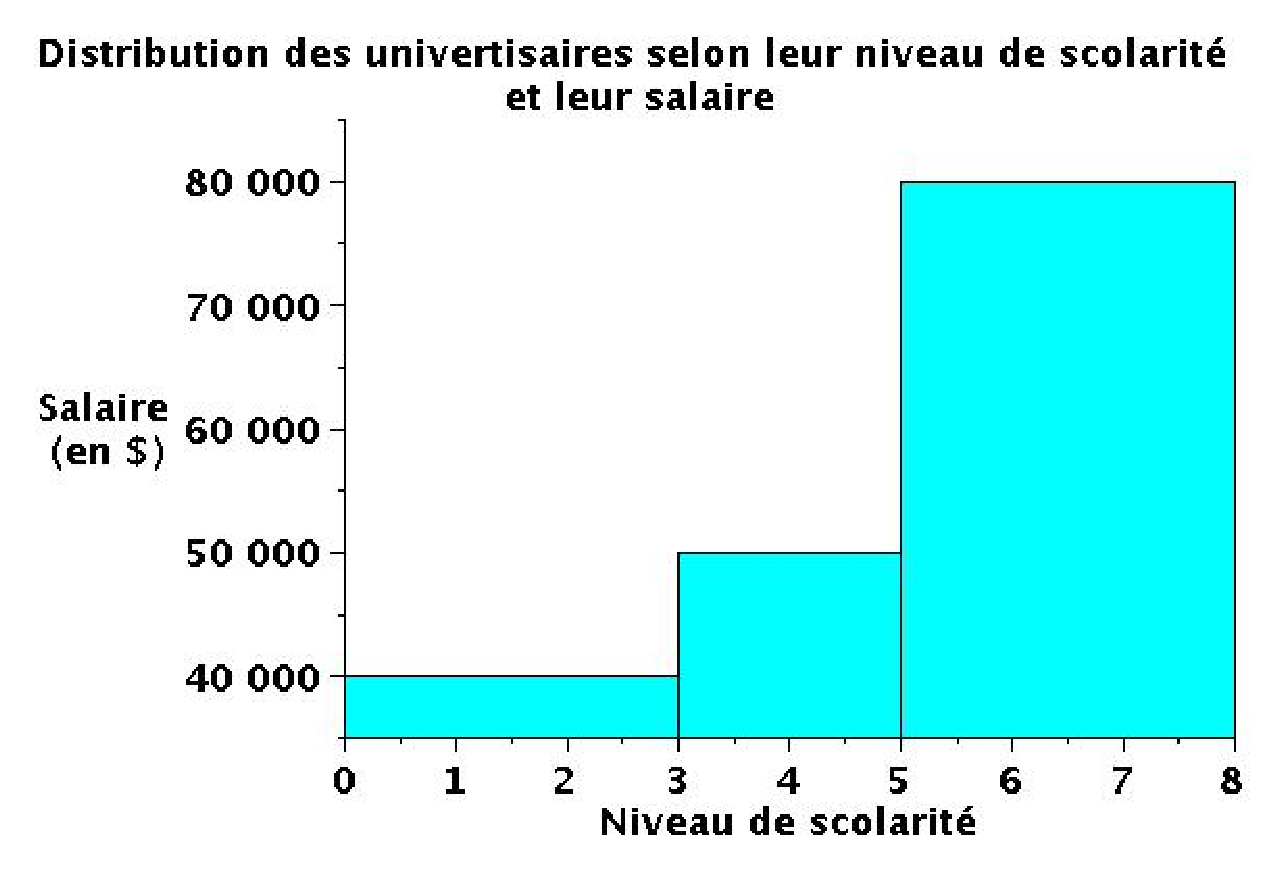
\includegraphics[width=8cm,bb=14 14 611 415]{Q2008v.eps}
 % Q2008v.eps: 1179666x1179666 pixel, 300dpi, 9987.84x9987.84 cm, bb=14 14 611 415
\end{center}

What type of graph is it?\\
a$)$ Bar graph\\
b$)$ Stem and leaf diagram\\
c$)$ Pie chart\\
d$)$ Histogram\\

Answer: d$)$\\

Explanation:
\begin{center}
 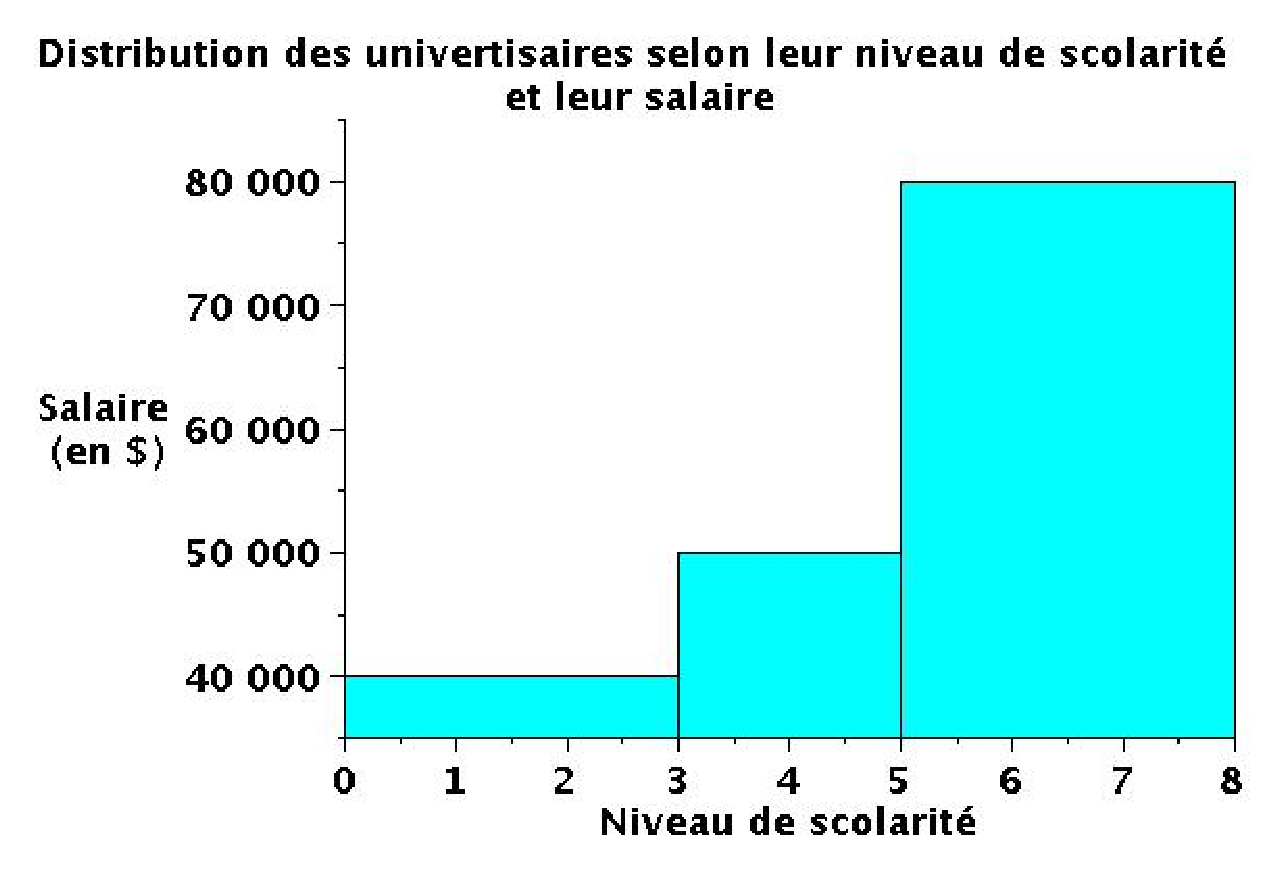
\includegraphics[width=8cm,bb=14 14 611 415]{Q2008v.eps}
 % Q2008v.eps: 1179666x1179666 pixel, 300dpi, 9987.84x9987.84 cm, bb=14 14 611 415
\end{center}
We want to know what type of graph this is.\\
\begin{itemize}
 \item Bar charts' bars are all the same width.\\
 \item Stem and leaf diagrams' bars are made of numbers.\\
 \item Pie charts are shaped like a circle.\\
 \item Histograms are made of bars that can have different widths and different heights.\\
\end{itemize}
Consequently, the answer is d).\\

2009-- In statistics, what is name given to the most frequent data collected?\\

a$)$ Frequency \\
b$)$ Median\\
c$)$ Fashion\\
d$)$ Mode\\

Answer: d$)$\\

Explanation:\\
In a data set, the most frequent data collected is called the mode.\\
Consequently, the answer is d).\\

%Questions statistiques mathematiques 416 difficulte 2
%Etudes statistiques

2010-- What is a statistical study that studies different characteristics of each member of a population called? \\

a$)$ A poll\\
b$)$ A census\\
c$)$ A survey\\
d$)$ A phone survey\\

Answer: b$)$\\

Explanation:\\
A census is a statistical study that looks at different characteristics of each member of a population. For example, if a small business owner wants to know how many years of experience and what kind of backgrounds his employees have, he must run a census. \\
Consequently, the answer is b).\\

2011-- Andreas wants to collect data to find out if the students are witnessing violence at his school. He says he can use a written questionnaire to collect his data. Is this true or false?\\

Answer: True\\

Explanation:\\
A written questionnaire is a method that may be used to collect data. \\
Consequently, the answer is : true.\\

%Echantillonnage (Sampling)

2012-- What sampling method can be used if the population is divided into groups? \\

a$)$ Simple random sampling.\\
b$)$ Stratified sampling.\\
c$)$ Cluster sampling.\\
d$)$ Group sampling.\\


Answer: c$)$\\

Explanation:\\
Cluster sampling is a sampling method in which the entire population is divided into groups, or clusters, and a random sample of these clusters is selected. All observations in the selected clusters are included in the sample.\\
Consequently, the answer is c).\\

2013-- One can use a sample that is non-representative of the population to extrapolate a poll's results. True or false? \\

Answer: False\\

Explanation:\\
A sample must be representative of the population to ensure the validity of a poll's results.\\
Consequently, the answer is: false.\\

%Quartiles

2014-- Here are the top 10 results of a French competition. What is the median of this data set?  \\
\begin{center}
 \begin{tabular}{|c  c  c  c  c|} \hline

95 & 95 & 96 & 96 & 96 \\
98 & 98 & 99 & 99 & 100 \\ \hline

\end{tabular}
\end{center}

Answer: 97\\

Explanation:\\
\begin{center}
 \begin{tabular}{|c  c  c  c  c|} \hline

95 & 95 & 96 & 96 & 96 \\
98 & 98 & 99 & 99 & 100 \\ \hline

\end{tabular}
\end{center}
Since the data set size is even, the median is the arithmetic mean of the 2 data points in the middle of the ordered data set. Since there are 10 values in the set, one must take the average of the fifth and the sixth value.\\
\begin{equation*}
 \frac{96+98}{2}=97
\end{equation*}
Consequently, the answer is 97.\\

2015-- Here are Catherine's best 10 high school marks. What is the value of the first quartile?
\begin{center}
 \includegraphics[width=6cm,height=8cm,angle=-90]{Q2015.eps}
 % Graph.eps: 1048576x0 pixel, 0dpi, infxnan cm, bb=
\end{center}


a$)$ 95\\
b$)$ 96\\
c$)$ 99\\
d$)$ 100\\

Answer: b$)$\\

Explanation:
\begin{center}
 \includegraphics[width=6cm,height=8cm,angle=-90]{Q2015.eps}
 % Graph.eps: 1048576x0 pixel, 0dpi, infxnan cm, bb=
\end{center}
We are looking for the first quartile value.\\
In the graph, quartiles are found by locating "whiskers". A whisker is a vertical mark in a box plot. The first whisker is located at 96.\\
Consequently, the answer is b).\\

%Mesures de position

2016-- The fifth rank is a position measurement. The first fifth rank is associated with:\\

a$)$ The five lowest results.\\
b$)$ The best results.\\
c$)$ The worst results.\\
d$)$ The first values of a set.\\

Answer: b$)$\\

Explanation:\\
When the fifth rank is used as a position measurement, the first fifth rank is associated to the best results.\\
Consequently, the answer is b).\\

2017-- Percentile is a position measurement. A value whose percentile is one is associated to: \\

a$)$ A central position in the data set.\\
b$)$ A median position in the data set.\\
c$)$ The best results.\\
d$)$ The worst results.\\

Answer: d$)$\\

Explanation:\\
When percentile is used as a position measurement, a percentile of one is associated with the worst results. Percentile indicates the percentage of data that is less than or equal to the considered value. \\
Consequently, the answer is d).\\

%Interpretation des donnees

2018-- Telworld is a phone company that offers services to its clients. Its president would like to offer more services. Since he wants to offer services that would be profitable to his company, he hires a survey firm to ask his clients about the particular needs they might have. What is the character of this survey? \\

a$)$ The number of phones per household.\\
b$)$ The particular needs of clients.\\
c$)$ The company's clients.\\
d$)$ The services used by clients.\\

Answer: b$)$\\

Explanation:\\
Character is what the statistical study is about. The purpose of this survey is to find out about the particular needs of the company's clients.\\
Consequently, the answer is b).\\

2019--  Mark volunteers at a local charity. During certain weeks, he works up to 10 hours, whereas during others, he doesn't work at all. Here is the frequency distribution of his working hours for the last 3 months. \\
\begin{center}
 \begin{tabular}{|c|c|} \hline
{\bf Number of hours} & {\bf Frequency}  \\ \hline \hline

[0-2] & 3 \\ \hline
]2-4] & 0 \\ \hline
]4-6] & 1 \\ \hline
]6-8] & 5 \\ \hline
]8-10] & 3 \\ \hline
\multicolumn{2}{c}{}\\
\end{tabular}\\
\end{center}


What is the modal class of distribution?\\

a$)$ [0-2]\\ [2mm]
b$)$ ]2-4]\\[2mm]
c$)$ ]4-6]\\[2mm]
d$)$ ]6-8]\\

Answer: d$)$\\

Explanation:\\
\begin{center}
 \begin{tabular}{|c|c|} \hline
{\bf Number of hours} & {\bf Frequency}  \\ \hline \hline

[0-2] & 3 \\ \hline
]2-4] & 0 \\ \hline
]4-6] & 1 \\ \hline
\textbf{]6-8]} & \textbf{5} \\ \hline
]8-10] & 3 \\ \hline
\multicolumn{2}{c}{}\\
\end{tabular}\\
\end{center}
The modal class of a distribution that is divided into classes is the class with the most elements in it. The answer is d).\\

%Questions statistiques mathematiques 416 difficulte 3
%Etudes statistiques

2020-- What kind of information about a data set can be obtained through a quartile graph?  \\

\begin{quote}
1. The data density \\
2. The spread of the data set\\
3. The average of the data set\\
4. The data frequency\\
\end{quote}

a$)$ 1 et 2\\
b$)$ 1 et 3\\
c$)$ 1 et 4\\
d$)$ 2 et 4\\

Answer: a$)$\\

Explanation:\\
Quartile graphs are used to find information about the density and the spread of a data set. However, they don't provide any information about the average or the frequency of the data points.\\
Thus, the answer is a).\\

2021-- In a statistical study, a sample is representative of the population if it has the same size as the population. True or false?\\

Answer: False\\

Explanation:\\
A sample is representative of the population if it possesses all the same characteristics of the population.\\
Thus, the answer is false.\\

%Echantillonnage

2022-- Karl is interested in finding out what kind of end of the year party the students at the school where he teaches would like to have. To choose the students he will interview, he takes his school phone book and calls every seventh student on each page. Which sampling method is he using?\\

a$)$ Random sampling\\
b$)$ Cluster sampling\\
c$)$ Stratified sampling\\
d$)$ Systematic sampling\\

Answer: d$)$\\

Explanation:\\
\begin{itemize}
 \item Random sampling consists in randomly choosing the whole set of people that make up the sample. \\
\item Cluster sampling is used when the population has been divided into groups. The sample is then the whole set of people that make up randomly selected groups.  \\
\item Stratified sampling consists in dividing the population into layers. Each layer is represented in the sample with the same ratio it is in the population. Finally, people are randomly selected in each layer to be part of the sample. \\
\item Systematic sampling consists in randomly choosing a first person and picking the other according to a pattern. \\
\end{itemize}
Therefore, the answer is d).\\

2023-- Lucy would like to know whether a question she has written for a poll is biased. The question is : \og Don't you think school should start at noon? \fg.\\
What do you think? \\

a$)$ Her question is biased.\\
b$)$ Her question is not biased.\\
c$)$ You think school should start at noon.\\
d$)$ A question cannot be biased.\\

Answer: a$)$\\

Explanation:
\begin{center}
 \og Don't you think school should start at noon?  \fg.
\end{center}
A question's formulation can be a source of bias. Lucy's question suggests to the respondent that she thinks school should start at noon. Therefore, it is biased. \\
The answer is a).\\

%Quartiles

2024-- Mark, Karl, Jan, and Eric are trying to make sense out of the following box plot:
\begin{center}
 \includegraphics[width=6cm,height=8cm,angle=-90]{Q2024.eps}
 % Q2024.eps: 1048576x0 pixel, 0dpi, infxnan cm, bb=
\end{center}

Whose statement is clearly false?\\

a$)$ Mark says that the interquartile range is 3.\\
b$)$ Karl says that the data is denser in the second quartile.\\
c$)$ Jan says that the median is 4.\\
d$)$ Eric says that the fourth quartile contains more data points. \\

Answer: d$)$\\

Explanation:\\
Eric is making a mistake by saying that the fourth quartile contains more data points, since, by definition, each quartile contains the same number of data points. \\
Thus, the answer is d).\\

2025-- Jonathan is given a box plot, but he does not have the data set that generated it. How can he compute the average of this data set?\\

a$)$ He must take the arithmetic mean of the maximum and the minimum of the data set.\\
b$)$ He must take the arithmetic mean of the minimum, the quartiles, and the maximum of the data set. \\
c$)$ He simply has to take the median of the data set. It is the same as the average.\\
d$)$ The average cannot be computed from the box plot. The actual data set is required.\\
\begin{center}
 \includegraphics[width=6cm,height=8cm,angle=-90]{Q2024.eps}
 % Q2024.eps: 1048576x0 pixel, 0dpi, infxnan cm, bb=
\end{center}

Answer: d$)$\\

Explanation:\\
Box plots are useful to get some general information about a data set, but the average cannot be deducted from it. The actual data set is required to do so.\\
Thus, the answer is d).\\

%Mesures de position

2026-- Jennifer is working in a women's clothing store. At the end
of the day, she looks at the sales totals, enters them in a computer
program, and makes a pie chart out of them.
\begin{center}
 \includegraphics[width=8cm]{Q2058b.eps}
 % Q2058b.eps: 1179666x1179666 pixel, 0dpi, infxinf cm, bb=
\end{center}
Her colleague Maude tells her that her pie chart is useless.\\
Why does she say that?\\

a$)$ Because Maude is rude.\\
b$)$ The pie chart shows the relative importance of a sale in relation to the other sales. It doesn't show the general state of the sales.\\
c$)$ The pie chart does not show the relative importance of a sale in relation to the other sales.\\
d$)$ The pie chart is not adapted for sales amounts.\\

Answer: b$)$\\

Explanation:\\
Maude says the pie chart is useless because it only shows the relative importance of a sale in respect to other sales. It does not show the general state of sales, which is the most relevant information in this situation.\\
Consequently, the answer b).\\

2027-- The data gathering process and the type of statistical study are the same thing. True or false?\\

Answer: False\\

Explanation:\\
The data gathering process is the mean taken to collect relevant information. The type of statistical study is the method used to study a population.\\
Thus, the answer is: false.\\

%Interpretation des donnees

2028-- A survey was conducted among a thousand men and women from
the province of Quebec to learn about their TV watching habits. Here
is the box plot that summarizes the answers to the question
concerning the number of hours weekly spent in front of the TV.
\begin{center}
 \includegraphics[width=6cm,height=8cm,angle=-90]{Q2028.eps}
 % Q2028.eps: 1048592x1048592 pixel, 0dpi, infxinf cm, bb=
\end{center}

Which statement is false?\\

a$)$ In average, the respondents watch TV 15 hours a week.\\
b$)$ There are as many respondents who watch TV between 0 and 10 hours a week as there are respondents who watch it between 10 and 15 hours a week.\\
c$)$ There are respondents who do not watch TV at all\\
d$)$ Half the respondents watch TV between 10 and 20 hours a week.\\

Answer: a$)$\\

Explanation:\\
It is not possible to determine a data set's average from a box plot.\\
Thus, the answer is a).\\

2029-- A survey was conducted among a thousand men and women from
Booktown to learn about their reading habits. Here is an histogram
summarizing the answers to the question asking them how many books
they read in a year.
\begin{center}
 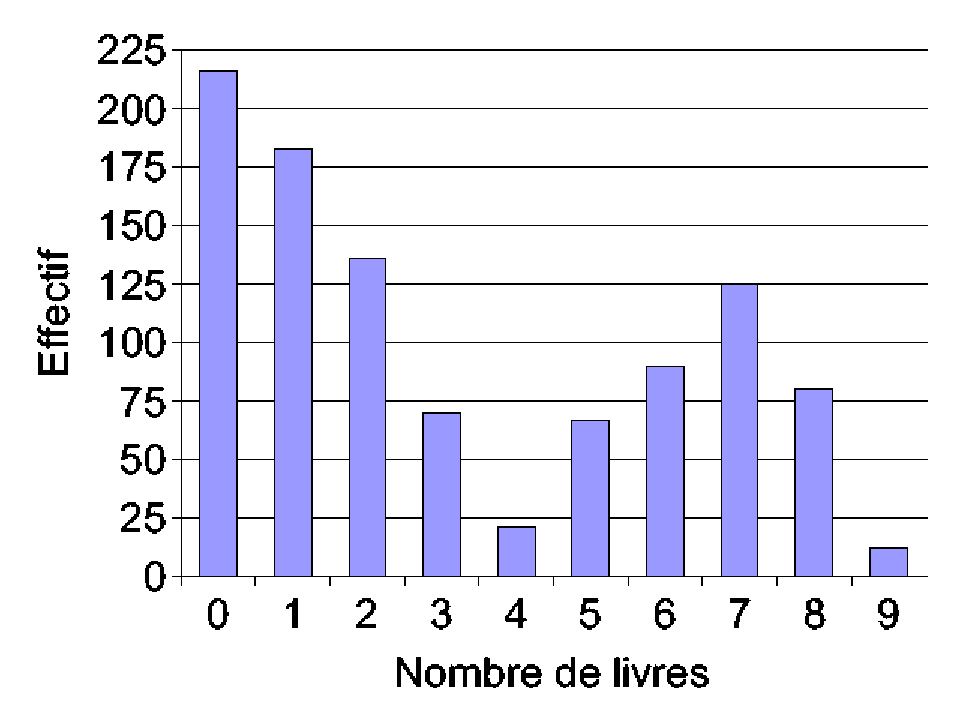
\includegraphics[width=6cm]{GraphLivreEPS.eps}
 % GraphLivreEPS.eps: 1048592x1048592 pixel, 0dpi, infxinf cm, bb=
\end{center}

Which statement is false?\\

a$)$ The mode of this distribution is 0 books.\\
b$)$ The mode of this distribution is between 200 and 225 books.\\
c$)$ More than half the respondents read 2 books or less a year.\\
d$)$ A large part of the respondents do not read any books during a year.\\

Answer: b$)$\\

Explanation:
\begin{center}
 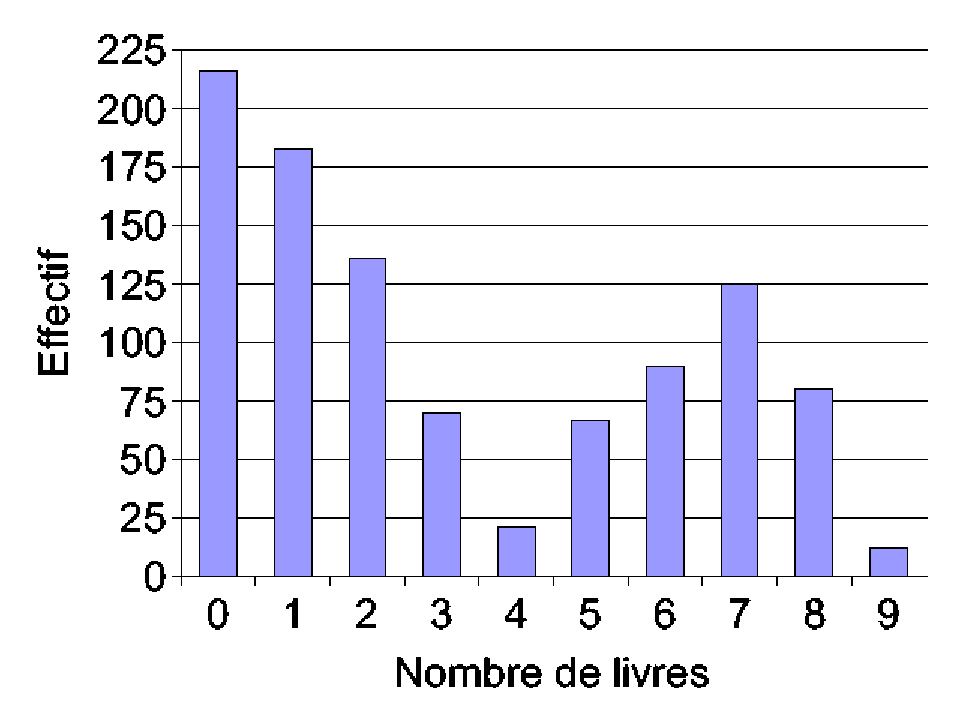
\includegraphics[width=6cm]{GraphLivreEPS.eps}
 % GraphLivreEPS.eps: 1048592x1048592 pixel, 0dpi, infxinf cm, bb=
\end{center}
We are looking for the false statement.\\
\begin{itemize}
 \item The mode of this distribution is 0 books.
 \item The mode of this distribution is between 200 and 225 books.
 \item More than half of the respondents read 2 books or less a year.
 \item A large part of the respondents do not read any books throughout the course of a year.\\
\end{itemize}
In a data distribution, the most frequent value is the mode. In this distribution, the mode is 0 and the mode's \textbf{frequency} is between 200 and 225 people.  \\
Thus, the answer is b).\\


\end{document}
